%Dies ist die Hauptseite des Dokumentes. Es werden u. a. alle Kapitel,
%Einstellung im Header eingebunden.
%Veränderungen müssen in folgenden Dateien vorgenommen werden:
      %- config.tex
      %- einzelne Kapitel (evtl. erweitern)

%Hier sind alle Einstellungen enthalten, die sich auf das Seiten- und
%Dokumentenlayout beziehen

\documentclass[
  11pt,                   % Schriftgröße
  DIV12,
  german,                 % für Umlaute, Silbentrennung etc.
  oneside,                % einseitiges Dokument
  titlepage,              % es wird eine Titelseite verwendet
  parskip=half,           % Abstand zwischen Absätzen (halbe Zeile)
  headings=normal,        % Größe der Überschriften verkleinern
  captions=tableheading,  % Beschriftung von Tabellen unterhalb ausgeben
  final                   % Status des Dokuments (final/draft)
]{scrreprt}               %


%------Ändern von Schriftschnitten - (Muss ganz am Anfang stehen !) ------------
\usepackage{fix-cm}


%------Umlaute -----------------------------------------------------------------
%   Umlaute/Sonderzeichen wie äüöß können direkt im Quelltext verwenden werden.
%    Erlaubt automatische Trennung von Worten mit Umlauten.
\usepackage[T1]{fontenc}
\usepackage[utf8]{inputenc}

%------Anpassung der Landessprache----------------------------------------------
\usepackage[ngerman]{babel}

%------Einfache Definition der Zeilenabstände und Seitenränder------------------
\usepackage{geometry}
\usepackage{setspace}

%------Schriftgrößenanpassung von einzelnen Textpassagen------------------------
\usepackage{relsize}

%------Trennlinien in Kopf- und Fusszeile
\usepackage[headsepline, footsepline, ilines]{scrpage2}

%------Grafiken und Farben -----------------------------------------------------
\usepackage{xcolor}
\usepackage{graphicx}

%------Packet zum Sperren, Unterstreichen und Hervorheben von Texten------------
\usepackage{soul}

%------ergänzende Schriftart----------------------------------------------------
\usepackage{helvet}

%------Lange Tabellen-----------------------------------------------------------
\usepackage{longtable}
\usepackage{array}
\usepackage{ragged2e}
\usepackage{lscape}

%------PDF-Optionen-------------------------------------------------------------
\usepackage[
  bookmarks,
  bookmarksopen=true,
  colorlinks=true,
  linkcolor=black,        % einfache interne Verknüpfungen
  anchorcolor=black,      % Ankertext
  citecolor=black,        % Verweise auf Literaturverzeichniseinträge im Text
  filecolor=black,        % Verknüpfungen, die lokale Dateien öffnen
  menucolor=black,        % Acrobat-Menüpunkte
  urlcolor=black,         % Farbe für URL-Links
  backref,                % Zurücktext nach jedem Bibliografie-Eintrag als
                          % Liste von Überschriftsnummern
  pagebackref,            % Zurücktext nach jedem Bibliografie-Eintrag als
                          % Liste von Seitenzahlen
  plainpages=false,       % zur korrekten Erstellung der Bookmarks
  pdfpagelabels,          % zur korrekten Erstellung der Bookmarks
  hypertexnames=false,    % zur korrekten Erstellung der Bookmarks
  linktocpage             % Seitenzahlen anstatt Text im Inhaltsverzeichnis verlinken
  ]{hyperref}






      % enthält eingebundene Packete

%------Seitenränder-------------------------------------------------------------
\geometry{verbose,                     % zeigt die eingestellten Parameter beim
                                       % Latexlauf an
      paper=a4paper,                   % Papierformat
      top=25mm,                        % Rand oben
      left=25mm,                       % Rand links
      right=25mm,                      % Rand rechts
      bottom=45mm,                     % Rand unten
      pdftex                           % schreibt das Papierformat in die
                                       % Ausgabe damit Ausgabeprogramm
                                       % Papiergröße erkennt
  }

%Seitenlayout
\onehalfspace        % 1,5-facher Abstand

%------Kopf- und Fußzeilen -----------------------------------------------------
\pagestyle{scrheadings}

%------Kopf- und Fußzeile auch auf Kapitelanfangsseiten ------------------------
\renewcommand*{\chapterpagestyle}{scrheadings}

%------Schriftform der Kopfzeile -----------------------------------------------
\renewcommand{\headfont}{\normalfont}

%----Spezielle Befehle
\newcommand{\lfk}[1]{$\langle LF#1\rangle$}

%----Farben
\definecolor{tubsRed}{cmyk}{0.1,1.0,0.8,0.0}
\definecolor{tuRed}{cmyk}{0.1,1.0,0.8,0.0}

%------Kopfzeile----------------------------------------------------------------
\setheadsepline{1pt}[\color{tuRed}]
\setlength{\headheight}{21mm}        % Höhe der Kopfzeile
\ihead{\large{\textsc{\praktikumTitel}}\\    % Text in der linken Box
       \small{\projektTitel}}
\chead{}                            % Text in der mittleren Box

%----Fusszeile
\setfootsepline{1pt}[\color{tuRed}]
\cfoot{}                            % Text in mittlerer Box
\ofoot{\pagemark}                    % Seitenzahl in rechter Box



%------Labels mit eigenem Text für \ref ----------------------------------------
\makeatletter
\def\namedlabel#1#2{\begingroup
#2%
\def\@currentlabel{#2}%
\phantomsection\label{#1}\endgroup
}
\makeatother


%------Neue Environments -------------------------------------------------------

\newcommand{\refsetcounter}[2]{\setcounter{#1}{#2}\addtocounter{#1}{-1}\refstepcounter{#1}}

%Funktion im Pflichtenheft
\newcounter{functioncount} 
\newenvironment{function}[2]{\refsetcounter{functioncount}{#1}\large\textbf{\sffamily{#2 }}\namedlabel{F#1}{$\langle F#1\rangle$}\normalsize\begin{description}\setlength{\itemsep}{-5pt}}{\end{description}}

%Daten im Pflichtenheft
\newcounter{datacount} 
\newenvironment{data}[2]{\refsetcounter{datacount}{#1}\textbf{#2} \namedlabel{D#1}{$\langle D#1\rangle$}\\}{}

%Kriterien im Pflichtenheft
\newcounter{mustcount} 
\newcommand{\must}[2]{\refsetcounter{mustcount}{#1}\namedlabel{RM#1}{$\langle RM#1\rangle$} #2\\}

\newcommand{\should}[2]{\refsetcounter{datacount}{#1}\namedlabel{RS#1}{$\langle RS#1\rangle$} #2\\}

\newcommand{\could}[2]{\refsetcounter{datacount}{#1}\namedlabel{RC#1}{$\langle RC#1\rangle$} #2\\}

\newcommand{\wont}[2]{\refsetcounter{datacount}{#1}\namedlabel{RW#1}{$\langle RW#1\rangle$} #2\\}

%Qualitätsanforderungen im Pflichtenheft
\newcommand{\qualityReq}[2]{\refsetcounter{datacount}{#1}\namedlabel{Q#1}{$\langle Q#1\rangle$} #2\\}

% Benutzeroberflächen im Pflichtenheft
\newcounter{uicount}
\newenvironment{ui}[2]{\refsetcounter{uicount}{#1}\textbf{#2} \namedlabel{UI#1}{$\langle UI#1\rangle$}\\}{}

% Klassen
\newcounter{classcount}
\newenvironment{class}[2]{\refsetcounter{classcount}{#1}\textbf{#2}\namedlabel{CL#1}{$\langle CL#1\rangle$}\begin{description}\setlength{\itemsep}{-5pt}}{\end{description}}

% Entitäten
\newcounter{entitycount}
\newenvironment{entity}[2]{\refsetcounter{entitycount}{#1}\textbf{#2} \namedlabel{E#1}{$\langle E#1\rangle$}\\}{}

% Component
\newcounter{componentcount}
\newenvironment{component}[2]{\refsetcounter{componentcount}{#1}\textbf{Komponente \namedlabel{C#1}{$\langle C#1\rangle$}: #2}\\}{}

% Interface
\newcounter{interfacecount}
\newenvironment{interface}[2]{\refsetcounter{interfacecount}{#1}\textbf{Schnittstelle \namedlabel{I#1}{$\langle I#1\rangle$}: #2}\\}{}

% Testfall
\newcounter{testcasecount}
\newenvironment{testcase}[2]{\clearpage\refsetcounter{testcasecount}{#1}\subsection{Testfall $\langle T#1\rangle$ - #2}\label{T#1}\begin{description}\setlength{\itemsep}{-5pt}}{\end{description}}
          % Diese Datei enthält alle
                                          % Layouteinstellungen
\newcommand{\dokumentTitel}{Angebot}
% Definition von globalen Parametern, die derzeit auf der Titelseite und in der
% Kopfzeile verwendet werden. Der in <> gesetzte Text ist zu verändern.

\newcommand{\praktikumTitel}{Das Gro\ss{}e SQL-Spiel}
\newcommand{\projektTitel}{The SQL-Alchemist}
\newcommand{\institut}{
	Institut f\"ur Informationssysteme\\
	Prof. Dr. Wolf-Tilo Balke\\
	M\"uhlenpfordtstra\ss{}e 23, 2.OG\\
	D-38106 Braunschweig\\
}
\newcommand{\institutsLogo}{common/ISF_Logo.pdf}
\newcommand{\betreuer}{Jan-Christoph Kalo}


%------Beginn des Gesamtdokumentes----------------------------------------------
\begin{document}

%------Eingebundene Seiten, Verzeichnisse bzw. Kapitel--------------------------
% Dies ist die Titelseite.
% Die Ausgabe darf 1 Seite nicht überschreiten, also ggf. Abstände anpassen
% Die Angabe in [...] gibt den Abstand nach der entsprechenden Zeile an.


%----Stil dieser Seite----------------------------------------------------------
\thispagestyle{plain}      % Kopfzeile bleibt leer

%----Beginn der Titelseite------------------------------------------------------
\begin{titlepage}

%----eingebundenes Logo der TU--------------------------------------------------
%\setlength{\unitlength}{1mm}
%  \begin{picture}(00,00)(+25,-04)
%  	\color{tuRed}
%    \put(055,006){\line(1,0){150}}
%    \put(005,000){
\includegraphics[width=6.3cm]{common/TUBraunschweig_4C.pdf}}
%    \put(150,010){\includegraphics[width=8cm,height=2.4cm,keepaspectratio]{\institutsLogo}}
%  \end{picture}\\[5ex]
%\hspace*{-2cm}


\vspace*{-3.8cm}
\hspace*{-2cm}\begin{minipage}{1.25\textwidth}

\includegraphics[width=6.3cm]{common/TUBraunschweig_4C.pdf}\setlength{\unitlength}{1mm}\begin{picture}(00,00)(0,0)\color{tuRed}\put(000,004){\line(1,0){150}}\end{picture}%\hfill
\parbox[b]{0.68\textwidth}{\hfill\includegraphics[width=8cm,height=2.4cm,keepaspectratio]{\institutsLogo}\\~}
\end{minipage}


~\\[4ex]

%----zentrierte Ausrichtung über die gesamte Seite----------------------------
\begin{center}

%----Titel des Praktikum (\praktikumTitel in newComments zu verändern)--------
{\relsize{4}{\textbf{\textsc{\praktikumTitel}}}}\\[4ex]

%----Titel des Teilprojektes (\projektTitel in newComments verändern)---------
{\relsize{3}{\textbf{\textsc{\projektTitel}}}}\\[4ex]

Software-Entwicklungspraktikum (SEP)\\
Sommersemester 2015\\[4ex]

{\relsize{3}{\textbf{\dokumentTitel}}}\\[2ex]

%----Daten des Auftraggebers
Auftraggeber:\\
Technische Universität Braunschweig\\
\institut[2ex]
Betreuer: \betreuer\\[2ex]

Auftragnehmer:\

% ----Tabelle der Praktikumsteilnehmer------------------------------------------
\begin{tabular}{l<{\hspace{20mm}} l<{\hspace{21mm}}}\\

  Name                   &   E-Mail-Adresse\\      % Zeilenüberschift

  \hline                    % Linie unterhalb der Zeilenüberschrift

  %----Nachfolgend alle Namen und E-Mail-Adressen der Teilnehmer einfügen
 
 Gabriel Ahlers &  g.ahlers@tu-braunschweig.de\\
 Majid Dashtiepielehroud &  m.dashtiepielehroud@tu-braunschweig.de\\
 Ronja Friebe &  r.friebe@tu-braunschweig.de\\  
 Stefan Hanisch &  stefan.hanisch@tu-braunschweig.de\\  
 Fabio Luigi Mazzone & f.mazzone@tu-braunschweig.de\\  
 Nicole Naczk &  n.naczk@tu-braunschweig.de\\  
 Denis Nagel &  denis.nagel@tu-braunschweig.de\\  
 Luca Porcello &  l.porcello@tu-braunschweig.de\\  
 Christian Reineke &  c.reineke@tu-braunschweig.de\\  
 Christian Sander &  christian.sander@tu-braunschweig.de\\  
 Carl Schiller &  c.schiller@tu-braunschweig.de\\  
 Levent Muzaffer \"Uner &  l.uener@tu-braunschweig.de\\  
 S\"oren van der Wall &  s.van-der-wall@tu-braunschweig.de\\  
 Daniel Wolfram &  d.wolfram@tu-braunschweig.de\\  


\end{tabular}

%Zur Vereinheitlichung sollten hier die TU Braunschweig Emailadressen benutzt werden. % enthält Tabelle der Praktikumsteilnehmer

\vfill
Braunschweig, \today

\end{center}
\end{titlepage}
                      % Titelseite

\tableofcontents                          % Inhaltsverzeichnis wird automatisch
                                          % generiert
\listoffigures                            % ebenso das Abbildungsverzeichnis

%----Kapitel des Feinentwurfs, die mit Inhalt zu füllen sind--------------------
%!TEX root = ../Angebot.tex

\chapter{Einleitung}

Im Folgenden wird zuerst das Motiv f\"ur das Projekt \glqq Das Gro\ss{}e SQL-Spiel\grqq~erl\"autert und anschlie{\ss}end werden Projektablauf, -umfang und -organisation sowie s\"amtliche technische Grundlagen als auch Richtlinien gekl\"art. Dabei wird grunds\"atzlich zwischen einem Back- sowie einem Front-End unterschieden. Das Back-End steht hierbei f\"ur die Serverkomponente der Software. Das Front-End beschreibt die gesamte Oberfl\"ache und Visualisierung der Software.

%!\textbf{Hinweis zu den Templates:}

\section{Ziel}

Das Ziel ist es, eine plattform\"ubergreifende, interaktive Spielesoftware zu entwickeln, um den Studenten der Pflichtveranstaltung \glqq Relationale Datenbanksysteme I (RDBI)\grqq~den Umgang mit der Datenbankanfragesprache SQL vorlesungsbegleitend spielerisch zu vermitteln. Sie soll ab dem Wintersemester 2015 vollst\"andig in den \"Ubungsbetrieb der Vorlesung integriert werden. 

Es soll eine M\"oglichkeit geschaffen werden, praktische Aspekte im Bereich der Datenbankanfragen zu \"uben, da dies im Rahmen einer Lehrveranstaltung viele verschiedene Schwierigkeiten mit sich bringt. Zum Einen kann theoretisches Verst\"andnis zwar gut vermittelt werden, jedoch ist es nur eingeschr\"ankt m\"oglich, gen\"ugend \"Ubungsmaterial zur Verf\"ugung zu stellen, damit eine komplexe Anfragesprache, wie SQL, ge\"ubt und somit auch verstanden werden kann.

Die Software soll genau diese M\"angel aufgreifen und beheben.


\section{Motivation} 

SQL hat die F\"ahigkeit komplexe, schwer nachvollziehbare Anfragen an eine Datenbank zu stellen. In der Theorie wird durchaus verstanden was hinter einer Datenbankanfrage steht, jedoch sind die Studenten meistens nicht in der Lage dies z\"ugig in der Sprache SQL auszudr\"ucken. Damit dieses verstanden werden kann, muss es permanent wiederholt und ge\"ubt werden. 
Zur \"Ubung von SQL sind jedoch kaum sinnvolle Tools vorhanden, die ohne gro{\ss}en Aufwand benutzt werden k\"onnen. 
Der Aufwand besteht darin, einen Datenbankserver zu installieren, zu konfigurieren, sich entsprechende Datenmodelle zu \"uberlegen und diese mit sinnvollen Daten zu verkn\"upfen.   
Es soll eine Software entwickelt werden, die die M\"oglichkeit bietet, dieses den Studenten zu erleichtern. Es wird eine komplett funktionsf\"ahige Applikation erstellt, die unkompliziert aus jedem Webbrowser aufrufbar sein wird.

Nun bietet die zu entwickelnde Software genau diese M\"oglichkeiten. Wie ist es dann aber m\"oglich die Studenten zu motivieren sich mit genau diesem Programm auseinander zu setzten um tats\"achlich SQL zu \"uben? Hier greift das Prinzip der \glqq Gamification\grqq. Mit Hilfe von spielerischen Aspekten in Form eines Mini-Spiels und t\"aglichen bzw. w\"ochentlichen Challenges sollen die Studenten motiviert werden. Durch immer wechselnde, zuf\"allig generierte Herausforderungen und damit verbundenen Erfolgserlebnissen sollen die User belohnt werden und somit zum regelm\"a{\ss}igen Gebrauch dieser App animiert werden.

%!TEX root = ../Angebot.tex

\chapter{Formale Grundlagen}


Das Back-End der Software wird in der Programmiersprache Java entwickelt. Zur Erstellung der grafischen Schnittstelle des Front-Ends wird die Skriptsrache JavaScript und die textbasierte Auszeichnungssprache HTML 5.0 verwendet.
Diese Aspekte werden in Punkt 5, den Entwicklungsrichtlinien dieses Dokumentes, detailierter aufgef\"uhrt.

Die in der Anwendung verwendete Sprache ist Englisch.
%!TEX root = ../Angebot.tex

\chapter{Projektablauf}

\section{Meilensteine}

Alle wichtigen Ereignisse, wie zum Beispiel Abgabefristen die vom Kunden oder der Projektleitung gesetzt werden, aber auch intern im Team gesetzte Fristen, werden 
in Meilensteinen zusammengefasst und in einer Tabelle wiedergegeben. Dabei ist bei jedem einzelnen Meilenstein jeweils die Vervollst\"andigung gemeint.
Jedes Dokument wird vor jeder offiziellen Abgabe dem Betreuer zur Kontrolle vorgelegt.

\begin{longtable}{|l|c|c|c|c|}
	\hline
	\textbf{Nummer} & \textbf{Meilenstein} & \textbf{Dokumente} & \textbf{Abgabetermin}\\ 
	\hline
	1  	&  Projektstart      &         -     &    13.04.15     \\ 
	\hline
	2	&  Angebot an Betreuer & Angebot & 20.04.15 \\
	 \hline
	3	& Serverapplikation initialisiert & - & 24.04.15 \\
	\hline
	4	& Angebot \"uber Redmine & Angebot & 24.04.15 \\
	\hline
	5	& Vervollst\"andigen der Spielidee &  - & 24.04.15 \\
	\hline
	6 	& Pflichtenheft an Betreuer &  Pflichtenheft & 06.05.15 \\ 
	\hline
	7 	& GUI des Front-Ends  & - & 07.05.15 \\
	\hline
	8 	& Userverwaltung & - & 07.05.15 \\
	\hline
	9 	& Pflichtenheft \"uber Redmine &  Pflichtenheft & 13.05.15 \\
	\hline
	10 	& Zwischenpr\"asentation  &  - & 15.05.15 \\
	\hline
	11 	& Fachentwurf an Betreuer &  Fachentwurf & 27.05.15 \\
	\hline
	12 	& Fachentwurf \"uber Redmine &  Fachentwurf & 03.06.15 \\	
	\hline
	13 	& Verwaltung f\"ur Benutzerrechte & - & 24.06.15 \\
	\hline
	14 	& Technischer Entwurf an Betreuer &  Technischer Entwurf & 24.06.15 \\
	\hline
	15 	& Softwaretests & - & 30.06.15 \\
	\hline
	16 	& Technischer Entwurf \"uber Redmine &  Technischer Entwurf & 01.07.15 \\
	\hline
	17 	& Fertigstellung Minigame & - & 24.06.15 \\
	\hline
	18 	& Testdokumentation an Betreuer &  Testdokumentation & 08.07.15 \\
	\hline
	19 	& Testdokumentation \"uber Redmine &  Testdokumentation & 15.07.15 \\
	\hline
	20 	& Pr\"asentationsvorbereitung & - & 20.07.15 \\
	\hline
	21 	& Fertige Version &  Quellcode, ... & 23.07.15 \\
	\hline
\end{longtable}

\section{Geplanter Ablauf}

Ein Teil des Teams startet das Projekt mit dem Ausformulieren des Produktangebots. W\"ahrenddessen beginnt das Gestaltungsteam ihren kreativen Prozess.
Ideenentwicklung und -austausch sowie N\"utzlichkeitsabw\"agung f\"uhren schnell zur fertigen Spielidee. Dieser Ablauf wird gleichzeitig genutzt, um zu pr\"ufen welche 
Werkzeuge (Frameworks, Entwicklungsumgebungen, etc.) genutzt werden, und sich mit diesen vertraut zu machen. Dabei werden auch schon erste Grafiken wie etwa 
f\"ur den Start-Screen und das Hauptmen\"u enstehen.

Das Back-End-Team nutzt die Zeit um die Serverapplikation zu erstellen. Desweiteren werden Ideen f\"ur ein Administrationstool sowie zur User- und Datenverwaltung 
gesammelt und umsetzbar strukturiert. Zwischenzeitig wird ein Papierprototyp entstehen, der die Grundz\"uge der zu erstellenden Applikation enth\"alt und das Team auf
einen gemeinsamen Stand bringt.

Sobald der Kunde, sowie der Betreuer das Angebot angenommen haben, beginnt der praktische Teil.

Das n\"achste Ziel wird sein, einen lauff\"ahigen Prototypen zu entwickeln.
Daf\"ur erstellen ausgew\"ahlte Mitglieder des Entwicklerteams das sogenannte Pflichtenheft, um festzuhalten, was von dem Projektteam alles geliefert werden muss.
Bis zur Fertigstellung des Prototypen und dessen Pr\"asentation wird weiterhin ein Fachentwurf erstellt und eingereicht.

Das Front-End-Team wird nun sowohl das Hauptmen\"u als auch das \glqq Alchemistenlabor\grqq~(den eigentlichen \glqq SQL-Vokabeltrainer\grqq) bearbeiten, damit der repr\"asentative 
Teil des Projekts m\"oglichst zur Zwischenpr\"asentation ausf\"uhrbar ist.
Parallel wird sich das Back-End-Team um die Nutzer- und Rechteverwaltung k\"ummern. 

Nach der Zwischenpr\"asentation werden der Projektdokumentation noch der Technische Entwurf und die Testprotokolle hinzugef\"ugt.
Um die dazugeh\"origen Software-Tests k\"ummert sich das Team in der letzten Etappe.

Zum Abschluss des Projektes wird eine kleinere Gruppe aus ausgew\"ahlten Mitgliedern noch f\"ur eine gute Pr\"asentation beim Tag der jungen Software-Entwickler 
(TDSE)  sorgen. 

Zur besseren \"Ubersicht dieser einzelnen Abl\"aufe ist ein Gantt-Diagramm erstellt worden.

\begin{figure}[ht]
\centering
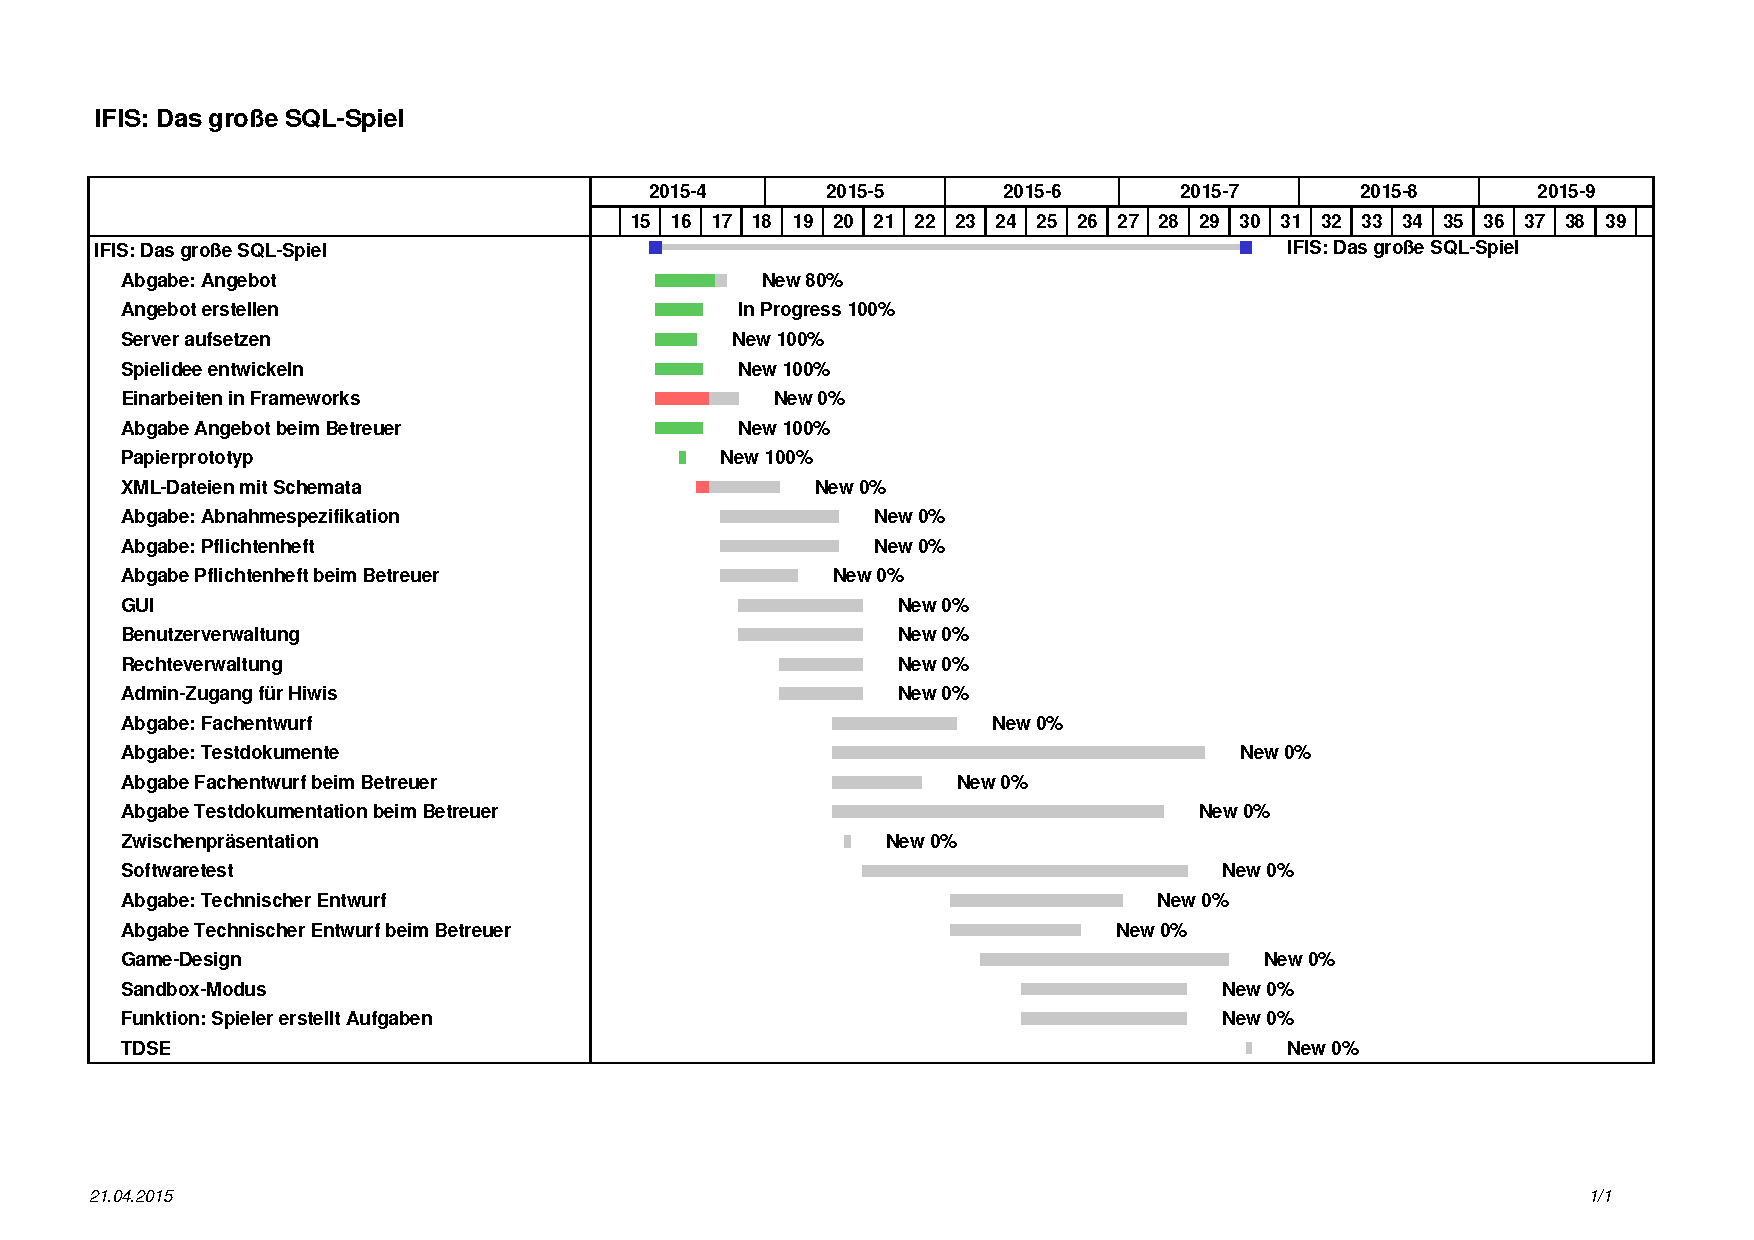
\includegraphics[height=\textwidth, angle=90]{figures/gantt.pdf}
\caption{Gantt-Diagramm}
\label{gantt}
\end{figure}
%!TEX root = ../Angebot.tex

% Kapitel 4
%-------------------------------------------------------------------------------

\chapter{Projektumfang}

\section{Lieferumfang}

Zum Lieferumfang der Software geh\"oren:

\begin{itemize}
	\item der Quellcode des Programms
	\item die ausf\"uhrbare Software
	\item die hinter der Nutzerschnittstelle liegende Datenbank
	\item das zugeh\"origes Handbuch
	\item die Spezifikation und der Entwurf der Software
	\item die Protokolle der Tests
	
\end{itemize}

\section{Kostenplan}

Die f\"ur das Projekt anfallenden Kosten, werden auf ca. 316.000 Euro gesch\"atzt. Davon entfallen
315.000 Euro auf den Lohn der Projektmitglieder (ausgehend von einem Arbeitslohn von 100 Euro pro Stunde und 30 Arbeitsstunden je Mitglied) 
und 1000 Euro auf den Kauf von Sprites, vorgefertigten Spieleger\"usten und weiteren f\"ur das Spiel ben\"otigten Objekten.

\section{Funktionaler Umfang}

Folgende Funktionen sollen in der abschlie{\ss}enden Version der Software enthalten sein:
\begin{enumerate}
	\item Insgesamt soll das Spiel dem Nutzer 3, beziehungsweise 4 verschiedene Modi bieten:
	\begin{enumerate}
      		\item Einen narrativen Modus, welcher dem Spieler erm\"oglicht in der Rolle des Alchemisten verschiedene Aufgaben zu 
			 erf\"ullen, um dann in der Geschichte des Spiels voranzuschreiten. Wobei es unabdingbar ist, dass der User
			 SQL-Anfragen \"ubt um in dem Modus weiter zu kommen.
		\item Einen Trivia-Modus, durch den die Spieler abseits eines festgelegten Handlungsstranges SQL-Abfragen \"uben 
			 k\"onnen,	indem sie zuf\"allig gestellte Aufgaben l\"osen.
		\item Einen Sandbox-Modus, der den Trivia-Modus durch vom Nutzer selbst erstellte Aufgaben erweitert. Diese Aufgaben 
			 stehen dann allen Nutzern zur Verf\"ugung und k\"onnen bewertet werden. Das Erstellen von Aufgaben jedoch bleibt freigeschalteten Spielern 
			 vorenthalten die sich im narrativen Modus bew\"ahrt haben. Dies wir durch das Back-End mit bestimmter Rechteverwaltung
			 realisiert.
		\item Einen Season-Modus, welcher von den Dozenten des Studienfaches RDBI genutzt werden kann, um die Software in den 
			 \"Ubungsbetrieb zu integrieren.
	\end{enumerate}
	\item Nutzerprofile und -statistiken, die den Fortschritt und die Erfolge eines jeden Spielers speichern. Au{\ss}erdem sollen diese grafisch
		aufbereitet werden und von jedem User abrufbar sein.
	\item Ranglisten, \"uber die sich die Nutzer untereinander vergleichen k\"onnen um die Motivation zu f\"ordern. 
		 Eventuell ist die Nutzung angemeldeten Spielern vorbehalten. 
	\item Ein Minispiel, welches sowohl im Story-, als auch im Trivia-Modus zum Einsatz kommt. Dabei handelt es sich um ein 
		 \glqq Jump \& Run\grqq-Spiel, in welchem die Spieler Gegenst\"ande einsammeln um Punkte zu erhalten und dabei 
		 SQL-Hindernisse \"uberwinden m\"ussen.
	\item Eine Benutzerverwaltung, die einzelne Rechte, sowie Rollen verwalten soll.
	\item Ein Admin-Tool, damit Dozenten und deren Mitarbeiter die Software in 
   		 ihre \"Ubungen integrieren k\"onnen. Insbesondere die Challenges, in dem Fall die Hausaufgaben, sollen hiermit erstellt und 
		 eingepflegt werden k\"onnen. Beim Erstellen von Hausaufgaben kann man einen Titel ausw\"ahlen und andere Eigenschaften
		 festsetzten. Zum Beispiel kann ein Zeit-Slot gesetzt werden in der die Hausaufgabe bearbeitet werden muss. 
	\item Auch die Studenten k\"onnen im Anschluss der Bearbeitung dieses Tool nutzen um zu \"uberpr\"ufen
		 ob sie die Hausaufgaben bestanden haben oder nicht. 
	\item Das Back-End bietet ebenfalls eine Schnittstelle an, die mit dem Software-Modul des Teamprojektes kommuniziert und es mit 
		entsprechenden XML-Schemata f\"ullt.
	\item Die Studenten bekommen die M\"oglichkeit Kommentare zu den Hausaufgaben abzugeben. Somit bekommt auch der Betreuer der
		Hausaufgaben eine Rewiew zum Schwierigkeitsgrad oder \"ahnlichen Kriterien. Auch dies wird durch das Back-End verwaltet.
\end{enumerate}




%!TEX root = ../Angebot.tex

\chapter{Entwicklungsrichtlinien}

\section{Konfigurationsmanagement}

Es gibt ein zentrales Repository auf Basis von Subversion (SVN), welches \"uber das Redmine des Instituts f\"ur Softwaretechnik und Fahrzeuginformatik (ISF) zur Verf\"ugung gestellt wird. Dieses Repository ist in drei Ordner unterteilt. In einem Ordner werden alle im Laufe des Projektes zu angefertigten Dokumente, die die Projektorganisation und den Kunden betreffen, abgelegt. Dazu z\"ahlen: ein Fachentwurf, eine Abnahmespezifikation, ein Pflichtenheft, ein technischer Entwurf, eine Testspezifikation und die entsprechenden Testprotokolle. Au{\ss}erdem gibt es zwei weitere Ordner, in die alle Dateien der jeweiligen Teilprojekte, das Back- sowie das Front-End, abgelegt werden. Hierbei handelt es sich unter anderem um Dateien mit dem Quellcode der jeweiligen Software-Komponente.  

Des Weiteren gibt es eine feste Kommentarstruktur, die bei jedem SVN-Commit, also dem Hochladen der ge\"anderten Dateien in das SVN-Repository, eingehalten werden soll. Dies f\"uhrt dazu, dass alle \"Anderungen nachvollziehbar, verst\"andlich und vollst\"andig sind. Um die Integrit\"at der Applikation zu gew\"ahrleisten, soll ebenfalls nur vollst\"andig ausf\"uhrbarer Code in das Repository hochgeladen werden.  


\section{Design- und Programmierrichtlinien}

F\"ur die Entwicklung des gesamten Projektes ist festgelegt, dass sich die Entwickler an folgende im Rahmen der Veranstaltung \glqq Software-Engineering I (SE I)\grqq~vorgestellten Coding-Guidelines halten:
\begin{itemize}
	\item Einr\"uckung: Um den Code \"ubersichtlicher zu gestalten, wird die Einr\"uckungstiefe auf 4 Zeichen festgelegt.
	\item Klammersetzung: Jede Klammer die zur Schlie{\ss}ung einer Methode bzw. einer Klasse gebraucht wird, wird in eine neue Zeile gesetzt. 
	\item Bezeichner: S\"amtliche Bezeichener (Parameter, Variablennnamen, Methodennamen, Klassennamen, etc.) werden sinnvoll nach ihrem Inhalt 		bennant, damit direkt ersichtlich ist, was die jeweilige Methode berechnet oder welche Information in jeder Variable steht.
	\item CamelCaseNotation: Zur besseren Lesbarkeit des Quelltextes werden Methoden in CamelCaseNotation notiert. 
	\item UPPER\_CASE Notation: Alle Konstanten werden in Gro{\ss}buchstaben, durch Unterstriche getrennt, geschrieben.
	\item lower\_case Notation: Imports und Packages werden in Kleinbuchstaben geschrieben.	
\end{itemize} 

Dar\"uber hinaus ist entschieden, s\"amtliche Kommentare auf Englisch zu verfassen.
Das Software-Dokumentationswerkzeug Javadoc generiert parallel aus dem Java-Quellcode eine vollst\"andige HTML-Dokumentationsdatei.

%!(Bestandteil des Java Development Kits) glossar


\section{Verwendete Software}

Als Entwicklungsumgebung wird IntelliJ IDEA von JetBrains verwendet, zum Erstellen von Diagrammen und technischen Zeichnungen  das Visualisierungsprogramm Dia, sowie Microsoft Visio. Textdokumente, die das Projekt betreffen, werden mit Hilfe des Software-Pakets LaTeX angefertigt und formatiert.

Das Front-End wird mithilfe der HTML5 Spiele-Engine melonJS und der plattformunabh\"angigen JavaScript-Bibliothek jQuery entwickelt, das Admin-Tool des Back-Ends mit dem Open-Source-Framework AngularJS und dem CSS-Framework Bootstrap.
F\"ur die Server-Komponente des Back-Ends wird das Web-Framework play! verwendet. 

Das Front-End-Team nutzt f\"ur das zu entwickelnde Mini-Spiel den Tiled Map Editor. Grafiken f\"ur die gesamte Software werden mit Hilfe des Bildbearbeitungsprogramm Adobe Photoshop CS6 entstehen.

Au{\ss}erdem wird eine Software des mitarbeitenden Teamprojektes, die automatisch Schemata generiert zur Verf\"ugung gestellt. Zudem kann auf eine Software, die im Rahmen einer Bachelorarbeit entwickelt wird, zur\"uckgegriffen werden, die sich mit der automatischen Generierung von SQL-Statements und Aufgabenstellungen besch\"aftigt.




%!TEX root = ../Angebot.tex

\chapter{Projektorganisation}

\section{Schnittstelle zum Auftraggeber}

Der Kunde steht den Entwicklern per Telefon-, E-Mail- und pers\"onlicher Kommunikation zur Verf\"ugung. Regelm\"a{\ss}ige
Meetings wurden direkt zu Anfang des Projektes auf donnerstags um 15 Uhr festgelegt.


\section{Schnittstelle zu anderen Projekten}

Die Mitglieder des externen Teamprojektes, die ihre Software zur Verf\"ugung stellen, und der Verfasser 
der Bachelorarbeit, dessen Software ebenfalls zur Verg\"ugung gestellt wird, k\"onnen sowohl \"uber die 
Projektbetreuer, als auch per E-Mail erreicht werden. 
Der Datenaustausch geschieht hierbei \"uber GitHub.

\section{Interne Kommunikation}

Das SEP-Team kommuniziert \"uber E-Mail bzw. Instant-Messenger und das eingerichtete Repository im Redmine.
Au{\ss}erdem finden sowohl mit den Betreuern und dem Kunden, als auch intern untereinander regelm\"a{\ss}ige Treffen statt.
Die Treffen werden mit dem Online-Termin-Planer Doodle organisiert.
Zur Protokollierung dieser Meetings wird ein webbasierter Editor von Google verwendet.


%\section{Kontaktdaten}

	
	
%!TEX root = ../Angebot.tex

\chapter{Glossar}

\begin{itemize}
	\item Back-End: Das Back-End bezeichnet eine Schicht eines Programms. Das Back-End verarbeitet zur Verf\"ugung gestellte Daten. Es entspricht hierbei der Serverkomponente des Programms.
	\item Front-End: Das Front-End ist das Gegenst\"uck zu dem Back-End. Es beschreibt Ausgabe des Programms und ist f\"ur eine entsprechende Visualisierung zust\"andig.
	\item Javadoc: Javadoc ist ein Software-Dokumentationswerkzeug, das aus Java-Quelltexten automatisch HTML- Dokumentationsdateien erstellt. 
	\item Redmine: Das Redmine ist eine webbasierte Organisations- und Projektverwaltungssoftware.
	%!\item Sprite: Ein Sprite ist ein zweidimensionales Grafikobjet. 
	\item Repository: Ein Repository ist ein verwaltetes Verzeichnis zur Speicherung von Daten
	\item Framework: Ein Framework ist ein vorgefertigtes Programmierger\"ust.
	\item Spiele-Engine: Eine Spiel-Engine ist ein spezielles Spiele-Framework, das den Spielverlauf steuert und f\"ur die Visualisierung des Spiels sorgt.  
\end{itemize}







%------Ende des Dokumentes------------------------------------------------------
\end{document}
